\section{Motivation}\label{sec:motivaiton}
Zu Beginn wurde durch eine Meinungsumfrage überprüft, ob bei Sprachassistenten mehr Datenschutz gewünscht ist. Dabei haben sich 110 Teilnehmer an der Umfrage beteiligt. Die Teilnehmer umfassten folgende Altersgruppen:
\begin{itemize}
	\item 1 bis 18 Jahre 
	\item 19 bis 25 Jahre
	\item 26 bis 35 Jahre
	\item 36 und älter	
\end{itemize}

55,5 \% der Teilnehmer waren männlich und 45,5\%  weiblich, wie in Abbildung \ref{fig:umfrage_teilnehmer} ersichtlich.

\begin{figure}[!h]
	\centering
	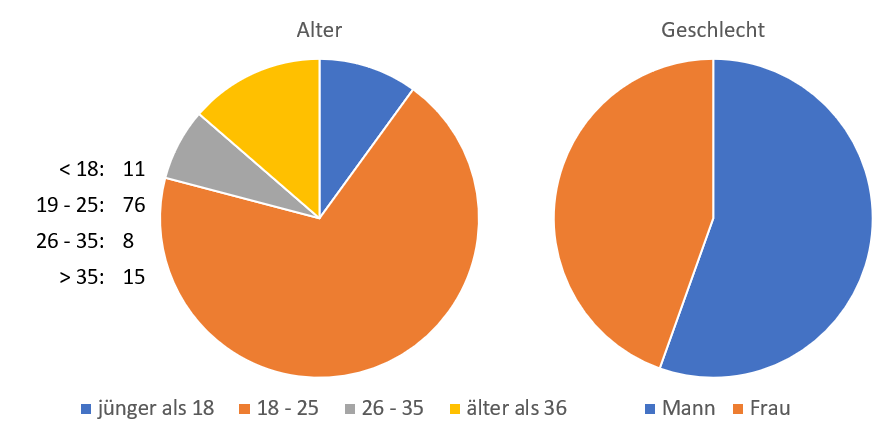
\includegraphics[width=0.9\linewidth]{Picture/umfrage_teilnehmer}
	\caption[Teilnehmer der Umfrage]{Teilnehmer der Umfrage}
	\label{fig:umfrage_teilnehmer}
	
\end{figure}

Den Teilnehmern wurden folgende Fragen gestellt:

\begin{enumerate}	
	\item Wie oft nutzen sie einen Sprachassistenten?
	\item Wissen sie was mit ihren Daten geschieht?
	\item Würden sie Geld für eine hohe Datensicherheit bezahlen?
	\item Wie viel Geld würden sie einmalig für eine hohe Datensicherheit einer Anwendung bezahlen?
	\item Bei welchen Anwendungen ist ihnen Privatsphäre besonders wichtig?	
\end{enumerate}

Bei der ersten Frage stellte sich heraus, dass 44,5\% einmal im Monat oder häufiger einen Sprachassistenten in Anspruch nehmen. In den USA wurde eine Studie von \glqq highervisibility\grqq{} durchgeführt, bei der mehr als 70\% der Teilnehmer einen Sprachassistenten mehr als einmal im Monat verwenden \cite{highervisibility}.
Ein direkter Vergleich der Umfrage mit der Studie aus der USA ist in Abbildung \ref{fig:umfrage_haeufigkeit} zu sehen.

\begin{figure}[!h]
	\centering
	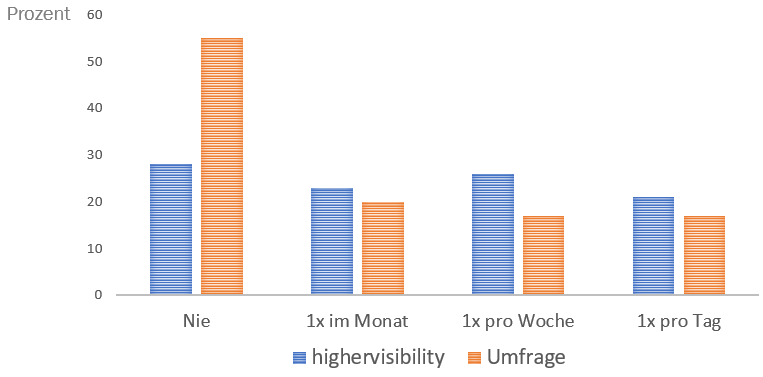
\includegraphics[width=0.9\linewidth]{Picture/umfrage_haeufigkeit}
	\caption[Nutzungshäufigkeit von Sprachassistenten]{Nutzungshäufigkeit von Sprachassistenten}
	\label{fig:umfrage_haeufigkeit}
\end{figure}

In der Studie wurden Menschen aus verschiedenen Altersgruppen und Herkunftsländern befragt. Die im Rahmen dieses Artikels durchgeführte Umfrage wurde überwiegend von jungen Leuten beantwortet.

\begin{figure}[!h]
 	\centering
 	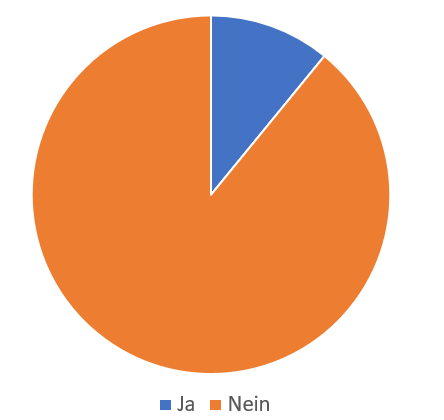
\includegraphics[width=0.5\linewidth]{Picture/umfrage_datenschutz}
 	\caption[Relevanz des Datenschutzes für die Umfrageteilnehmer]{Relevanz des Datenschutzes für die Umfrageteilnehmer}
 	\label{fig:umfrage_datenschutz}
\end{figure}

\newpage

Wie in Abbildung \ref{fig:umfrage_datenschutz} zu sehen ist, wissen 90\% der Teilnehmer nicht, was mit ihren Daten passiert. Die Zahlungsbereitschaft für Datensicherheit ist nach Altersgruppen in Abbildung \ref{fig:umfrage_geld_gruppen} visualisiert. Jeder Vierte würde für eine bessere Datensicherheit bezahlen und 56\% der Teilnehmer sind unsicher, ob sie dafür Geld ausgeben würden. Die Altersbetrachtung nach der Zahlungsbereitschaft ist bei der Gruppe unter 18 Jahren am geringsten. Die Schnittmenge der Teilnehmer, welche \glqq Ja\grqq{} oder \glqq Vielleicht\grqq{} angekreuzt haben, steigt mit zunehmendem Alter.

\begin{figure}[!h]
	\centering
	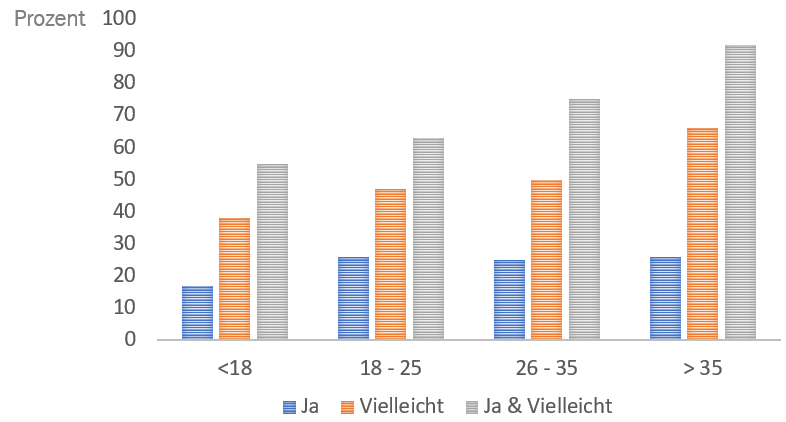
\includegraphics[width=0.9\linewidth]{Picture/umfrage_geld_gruppen}
	\caption[Zahlungsbereitschaft der Teilnehmer in verschiedenen Altersgruppen]{Zahlungsbereitschaft der Teilnehmer in verschiedenen Altersgruppen}
	\label{fig:umfrage_geld_gruppen}
\end{figure}

Der Betrag, welche die Teilnehmer für Anwendungen ausgeben würden variiert sehr und ist in Abbildung \ref{fig:umfrage_betrag} einzusehen. Ungefähr 15\% der befragten Teilnehmer sind nicht bereit dafür zu zahlen, während ein Großteil diese Bereitschaft hat.

\begin{figure}[!h]
	\centering
	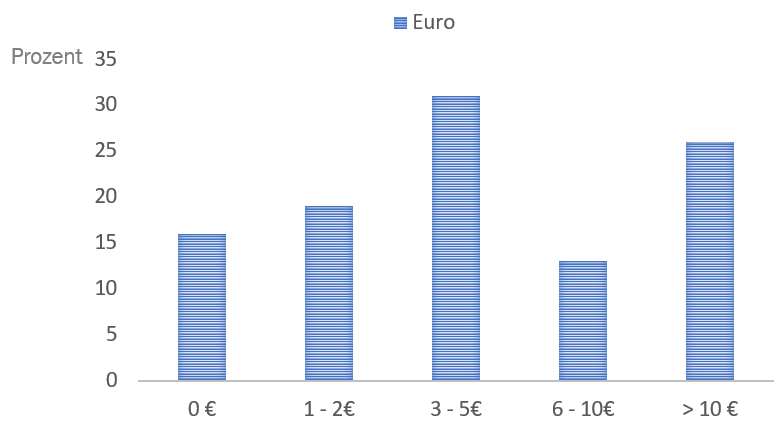
\includegraphics[width=0.9\linewidth]{Picture/umfrage_betrag}
	\caption[Zahlungsbereitschaft der Teilnehmer nach Betrag]{Zahlungsbereitschaft der Teilnehmer nach Betrag}
	\label{fig:umfrage_betrag}
\end{figure}

Wie Abbildung \ref{fig:umfrage_anwendung} zeigt, ist den Teilnehmern die Privatsphäre im Bereich Banking, Haussteuerung, Handysteuerung, Soziale Netzwerke und Chatting besonders wichtig.

Somit lassen sich folgende Schlussfolgerungen aus der Umfrage ziehen:
\begin{itemize}	
	\item Sprachassistenten werden in unterschiedlichem Umfang genutzt
	\item Die Nutzer wissen nicht, was mit ihren Daten geschieht
	\item Nutzer würden für den Schutz ihrer Daten bezahlen
	\item Datenschutz ist in den Bereichen Banking, Chatting, Haussteuerung, Social Media und Handysteuerung wichtig.
\end{itemize}

\begin{figure}[!h]
	\centering
	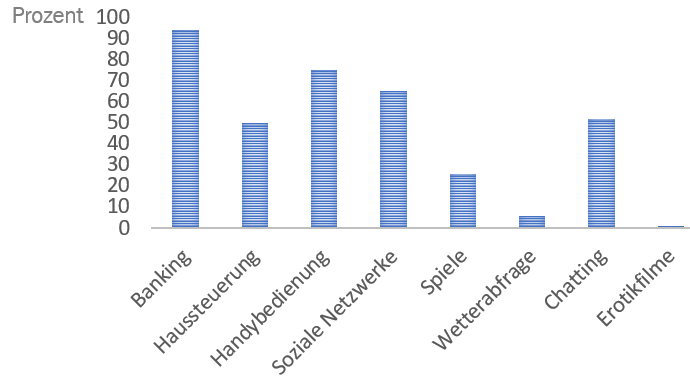
\includegraphics[width=0.9\linewidth]{Picture/umfrage_anwendung}
	\caption[Datenschutzrelevante Anwendungen der Umfrageteilnehmers]{Datenschutzrelevante Anwendungen der Umfrageteilnehmer}
	\label{fig:umfrage_anwendung}
\end{figure}
